\documentclass{emulateapj}
%\documentclass[12pt,preprint]{aastex}

\usepackage{graphicx}
\usepackage{float}
\usepackage{amsmath}
\usepackage{epsfig,floatflt}
\usepackage{hyperref}
\usepackage[toc, page]{appendix}
\usepackage{verbatim, amsmath, amsfonts, amssymb, amsthm}
\usepackage[utf8]{inputenc}
\usepackage{textcomp}
\usepackage{float}
\usepackage{xcolor}
\usepackage{color}
\usepackage{listings}
\usepackage{fancyhdr}
\usepackage[T1]{fontenc}
\usepackage{url}
\usepackage[export]{adjustbox}
\usepackage{calc}

\usepackage{accents}
\newcommand{\dbtilde}[1]{\accentset{\approx}{#1}}
\newcommand{\vardbtilde}[1]{\tilde{\raisebox{0pt}[0.85\height]{$\tilde{#1}$}}}

\usepackage{lipsum}
\usepackage[para]{footmisc}


\definecolor{mygreen}{rgb}{0,0.6,0}
\definecolor{mygray}{rgb}{0.5,0.5,0.5}
\definecolor{mymauve}{rgb}{0.58,0,0.82}

\lstset{ %
	backgroundcolor=\color{white}\ttfamily\tiny,   % choose the background color; you must add \usepackage{color} or \usepackage{xcolor}; should come as last argument
	basicstyle=\tiny,        % the size of the fonts that are used for the code \footnotesize,
	breakatwhitespace=false,         % sets if automatic breaks should only happen at whitespace
	columns=fullflexible,    %no spaces between columns
	keepspaces=true,
	breaklines=true,                 % sets automatic line breaking
	breakatwhitespace=true,
	captionpos=b,                    % sets the caption-position to bottom
	commentstyle=\color{mygreen},    % comment style
	deletekeywords={...},            % if you want to delete keywords from the given language
	escapeinside={\%*}{*)},          % if you want to add LaTeX within your code
	extendedchars=true,              % lets you use non-ASCII characters; for 8-bits encodings only, does not work with UTF-8
	frame=single,	                   % adds a frame around the code
	keepspaces=true,                 % keeps spaces in text, useful for keeping indentation of code (possibly needs columns=flexible)
	keywordstyle=\color{blue},       % keyword style
	language=Python,                 % the language of the code
	morekeywords={*,...},           % if you want to add more keywords to the set
	%numbers=left,                    % where to put the line-numbers; possible values are (none, left, right)
	%numbersep=5pt,                   % how far the line-numbers are from the code
	%numberstyle=\tiny\color{mygray}, % the style that is used for the line-numbers
	rulecolor=\color{black},         % if not set, the frame-color may be changed on line-breaks within not-black text (e.g. comments (green here))
	showspaces=false,                % show spaces everywhere adding particular underscores; it overrides 'showstringspaces'
	showstringspaces=false,          % underline spaces within strings only
	showtabs=false,                  % show tabs within strings adding particular underscores
	stepnumber=1,                    % the step between two line-numbers. If it's 1, each line will be numbered
	stringstyle=\color{mymauve},     % string literal style
	tabsize=1,	                   % sets default tabsize to 2 spaces
	%title=\lstname                   % show the filename of files included with \lstinputlisting; also try caption instead of title
}

\begin{document}

\title{Comparing efficiency of different algorithms for solving sets of linear equations}

\author{Bruce Chappell and Markus Bjørklund}

\email{markus.bjorklund@astro.uio.no}

\altaffiltext{1}{Institute of Theoretical Astrophysics, University of
  Oslo, P.O.\ Box 1029 Blindern, N-0315 Oslo, Norway}

\begin{abstract}
In this letter we investigate numerical solutions to Eigenvalue problems, specifically the buckling beam two point boundary value problem and the Schrödinger equation in one dimension.

\end{abstract}
\keywords{Jacobi method --- Linear algebra: Eigensolvers --- methods: computational}

\section{Introduction}
\label{sec:introduction}
\underline{\textbf{Reasons for project and overview of report}}

\section{Method}
\label{sec:method}
\underline{\textbf{Mostly the theory, math, and algorithms}}

This section will describe the methods we utilized to acquire our results.

\subsection{Theoretical model}

\subsubsection{The Schrödinger equation}

Note: Some steps will be skipped here. A full derivation can be found in \cite{Project}.

The radial part of the Schrödinger equation is given by

\begin{equation}
  -\frac{\hbar^2}{2 m} \left ( \frac{1}{r^2} \frac{d}{dr} r^2
  \frac{d}{dr} - \frac{l (l + 1)}{r^2} \right )R(r)
     + V(r) R(r) = E R(r).
\end{equation}

We consider the case of the harmonic oscillator potential, which has $V(r) = (1/2)kr^2$ with $k=m\omega^2$, where $E$ is the energy and $\omega$ is the oscillator frequency.

With the substitutaion $R(r) = (1/r) u(r)$ we obtain

\begin{equation}
  -\frac{\hbar^2}{2 m} \frac{d^2}{dr^2} u(r)
       + \left ( V(r) + \frac{l (l + 1)}{r^2}\frac{\hbar^2}{2 m}
                                    \right ) u(r)  = E u(r) .
\end{equation}

Now in spherical coordinates we have $r\in [0,\infty)$ and boundary conditions $u(0)=0$ and $u(\infty)=0$.

For the case of a repulsive Coulomb interaction, we get the result

\begin{equation}
\left(  -\frac{\hbar^2}{m} \frac{d^2}{dr^2}+ \frac{1}{4}k r^2+\frac{\beta e^2}{r}\right)\psi(r)  = E_r \psi(r).
\end{equation}

\subsubsection{Scaling the equations}
To simplify the problem, we scale the equations. We introduce the variable $\rho = \frac{r}{\alpha}$, where $\alpha$ is a constant. Introducing this into the equations, and requiring that

\begin{equation}
\frac{mk}{\hbar^2} \alpha^4 = 1,
\end{equation}

 as well as defining

 \begin{equation}
\lambda = \frac{2m\alpha^2}{\hbar^2}E,
\end{equation}

we arrive at

\begin{equation}
  -\frac{d^2}{d\rho^2} u(\rho) + \rho^2u(\rho)  = \lambda u(\rho),
\end{equation}

for the case of one electron. For the case of two electrons with a repulsive Coulomb interaction, we also define a frequency

\begin{equation}
\omega_r^2=\frac{1}{4}\frac{mk}{\hbar^2} \alpha^4,
\end{equation}

fix the constant $\alpha$ by

\begin{equation}
\frac{m\alpha \beta e^2}{\hbar^2}=1
\end{equation}

and introducing

\begin{equation}
\lambda = \frac{m\alpha^2}{\hbar^2}E,
\end{equation}

we arrive at

\begin{equation}
  -\frac{d^2}{d\rho^2} \psi(\rho) + \omega_r^2\rho^2\psi(\rho) +\frac{1}{\rho} = \lambda \psi(\rho).
\end{equation}

\subsection{Numerical model}
We will discretize the problem to reduce it to an Eigenvalue problem. We divide our variable $\rho$ into N points, and define a step length h as

\begin{equation}
  h=\frac{\rho_N-\rho_0 }{N}.
\end{equation}

We then get a discretized variable $rho_i$, given by
\[
    \rho_i= \rho_0 + ih \hspace{1cm} i=1,2,\dots , N.
\]
Using the approximation

\begin{equation}
    \frac{d^2}{d\rho^2} u(\rho) =\frac{u(\rho+h) -2u(\rho) +u(\rho-h)}{h^2} +O(h^2),
    \label{eq:diffoperation}
\end{equation}

for the second derivative, and using shorthand notation, we can write the Schrödinger equation as

\begin{equation}
-\frac{u_{i+1} -2u_i +u_{i-1} }{h^2}+V_iu_i  = \lambda u_i
\end{equation}

We define the diagonal elements d as
\begin{equation}
   d_i=\frac{2}{h^2}+V_i,
\end{equation}

where we have $V_i = \rho^2$ for the case of one electron, and $V_i = \omega_r^2 \rho^2 + \frac{1}{\rho}$ for the case of the repulsive Coulomb interaction. The non-diagonal matrix elements given as

\begin{equation}
   e_i=-\frac{1}{h^2}.
\end{equation}

This simplifies the equation further, and it reduces to

\begin{equation}
d_iu_i+e_{i}u_{i-1}+e_{i}u_{i+1}  = \lambda u_i,
\end{equation}

We get the Eigenvalue equation $\mathbf{A}\vec{u} = \lambda \vec{u}$, with $\mathbf{A}$ given as

\begin{equation}
    \mathbf{A} =
    \begin{bmatrix}d_1 & e_1 & 0   & 0    & \dots  &0     & 0 \\
                                e_1 & d_2 & e_2 & 0    & \dots  &0     &0 \\
                                0   & e_2 & d_3 & e_3  &0       &\dots & 0\\
                                \dots  & \dots & \dots & \dots  &\dots      &\dots & \dots\\
                                0   & \dots & \dots & \dots  &\dots  e_{N-3}     &d_{N-2} & e_{N-2}\\
                                0   & \dots & \dots & \dots  &\dots       &e_{N-2} & d_{N-1}
             \end{bmatrix}
      \label{eq:sematrix}
\end{equation}

\subsubsection{Unitary transformations}
Unitary or orthogonal transformations have the property of conserving the dot product and orthogonality. We will show this for orthogonal matrices, but the argument extends to unitary transformations in the complex domain.

Suppose we have two vectors $\bold{v}_i$ and $\bold{v}_j$. Now, if we consider a orthogonal matrix $\bold{U}$, it has the property that $\bold{U}^T = \bold{U}^{-1}$ such that $\bold{U}^T\bold{U} = \bold{U}\bold{U}^T = \bold{I}$. Applying the transformation, we get new vectors $\bold{w}_i = \bold{U}\bold{v}_i$ and $ \bold{w}_j = \bold{U}\bold{v}_j$.
Now let's consider the dot product between these new vectors:

\begin{align*}
	\bold{w}_i \boldsymbol{\cdot} \bold{w}_j &= \left(\bold{U}\bold{v}_i\right) \boldsymbol{\cdot} \left(\bold{U}\bold{v}_j\right) \\
	&= \left(\bold{U}\bold{v}_i\right)^T \left(\bold{U}\bold{v}_j\right) \\
	&= \bold{U}^T \bold{v}_i^T \bold{U}\bold{v}_j \\
	&= \bold{v}_i^T  \bold{v}_j \bold{U}^T \bold{U} \\
	&= \bold{v}_i^T  \bold{v}_j \bold{I},
\end{align*}
which finally gives us

\begin{equation} \label{eq:dot}
	\bold{w}_i \boldsymbol{\cdot} \bold{w}_j = \bold{v}_i \boldsymbol{\cdot} \bold{v}_j.
\end{equation}


This shows the dot product is conserved. If we also assume that $\bold{v}_i$ and $\bold{v}_j$ is part of an orthogonal basis, such that $\bold{v}_i \boldsymbol{\cdot} \bold{v}_j = \delta_{ij}$, then we from equation \ref{eq:dot} that $\bold{w}_i \boldsymbol{\cdot} \bold{w}_j = \delta_{ij}$ is also true.

\subsubsection{Jacobi's rotation algorithm}
We are now ready to implement our solver. Using the above result, we know that similarity transformations will conserve the Eigenpairs of the equation. The idea is to apply multiple rotation matrices

\[\mathbf{S}_n^T\mathbf{S}_{n-1}^T...\mathbf{S}_1^T\mathbf{A}\mathbf{S}_1\mathbf{S}_2...\mathbf{S}_n\]

such that A eventually becomes diagonalized. To find these rotation matrices, we use the equations

\begin{equation}
  t = -\tau \pm \sqrt{1+\tau^2},
\end{equation}

\begin{equation}
   c = \frac{1}{\sqrt{1+t^2}},
\end{equation}
and
\begin{equation}
    s = tc,
\end{equation}
where we have defined $\tan\theta = t= s/c$, with $s=\sin\theta$ and $c=\cos\theta$ and
\begin{equation*}
    \cot 2\theta=\tau = \frac{a_{ll}-a_{kk}}{2a_{kl}}.
\end{equation*}

It can be shown, if you choose to zero out the largest off-diagonal element, that the norm of the new off-diagonal elements after rotation is smaller than the reduction in the off-diagonal element we're trying to zero out. Therefore, Jacobi's algorithm will always tend to all off-diagonal elements eventually being zero.

\section{Methods}
\label{sec:methods}
\subsection{Algorithm}
The program used to solve these eigenvalue problems uses a class to create an object that has methods to build the Toplitz matrix and implement Jacobi's Method. The methods programmed to perform the rotation are heavily based off of code found in [1].  After obtaining the eigeinvalues and eigenvectors for a given potential, number of iterations, and $\rho_{max}$, we plotted the first eigenvectors and repeated for different parameters. We also implemented a function to compare the computing time for Jacobi's Method and the Numpy linalg.eig function. This function compared the two times for the buckling beam problem for matrices of varying size. Another class was also used to create a fixed $4x4$ matrix which could then be used in our unit tests.
\subsection{Parameter Selection}
As specified in in section 2.1.1, the Schrödinger equation has Dirichlet boundary conditions of $u(0)=0$ and $u(\infty)=0$. This requires us to approximate $\infty$ with a given $\rho_{max}$. From Eq 11, step size is dependent on both $\rho_{max}$ and $N$, requiring and intelligent choice for both parameters when solving for potentials with different values of $\omega$. Through a process of trial and error we found the following $\rho_{max}$ values and $N = 100$ to offer a compromise between speed and resolution:
\begin{center}
\begin{tabular}{ |c|c|c|c|c| }
\hline
$\omega$ & 0.01 & 0.5 & 1 & 5 \\
\hline
$\rho_{max}$ & cell2 & cell3 & cell4 & cell5 \\
\hline
\end{tabular}
\end{center}
\subsection{Unit Tests}
To ensure or code was functioning properly, we implemented two unit tests at the beginning of the main program. The first unit test performed the $offdiagmax$ on a hard coded matrix with a max element at [0,3] and checked to make sure the function returned the right index for the maximum element. This is shown in the psuedo code bellow:
\begin{lstlisting}[language=Python]
def diagonal_unit_test():
    A = Test_object()
    A.build_test
    max_index = A.offdiagmax
    if (max_index[0] != 0 and max_index[1] != 3):
        print('Max index finder not function, test failed')
        exit()
    else:
        print('Max index finder working')
\end{lstlisting}
In addition, we wrote a unit test to ensure Jacobi's method was working properly by testing the orthogonality of the resulting eigenvectors and comparing the eigenvalues against those produced by Numpy's linalg.eig function.

\section{Results}
\label{sec:results}
We found Jacobi's method to be extremely slow compared to Numpy's eigenvalue solver as shown below.
\begin{figure}[H]
    \centering
    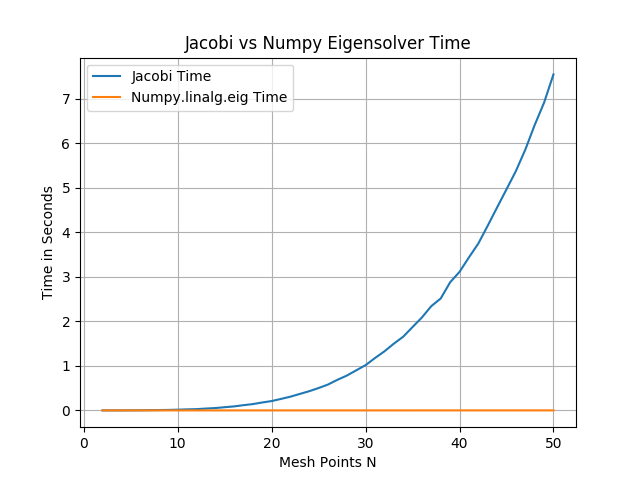
\includegraphics[scale=0.5]{jacobi_numpy_time.png}
    \caption{Solving time for the two methods plotted as function of matrix mesh points}
    \label{fig:1}
\end{figure}






\section{Conclusions}
\label{sec:conclusions}
\underline{\textbf{What we have supposed to have learned}}
\underline{\textbf{and the ideas the results should have confirmed}}
\subsection{Further research}
\underline{\textbf{Silly section, pretending to be real researchers}}
\\
\\
\\
\newpage
\begin{thebibliography}{}
\bibitem{Lecture}[(Hjorth-Jensen, 2018)]{MHJ} Hjorth-Jensen, Morten \, Sep 15 2017, "Computational Physics Lectures:Eigenvalue problems" , http://compphysics.github.io/ComputationalPhysics/doc/pub/eigvalues/pdf/eigvalues-print.pdf

\bibitem{Project}[(Hjorth-Jensen, 2018)]{MHJ} Hjorth-Jensen, Morten \, Sep 6 2018, "Project 2"
http://compphysics.github.io/ComputationalPhysics/doc/Projects/2019/Project2/pdf/Project2.pdf

\end{thebibliography}

\section{Appendix}
All source code, data and figures can be found at the github repository: https://github.com/bruce-chappell/FYS4150/tree/master/project1

\end{document}
